
% C. Wohlin, P. Runeson, M. H ̈ost, M. C. Ohlsson, B. Regnell, and A. Wessl ́en. Experimentation in Software Engineering. Springer Science & Business Media.
% M. Oivo, P. Kuvaja, P. Pulli, and J. Simil ̈a. Software engineering research strategy: Combining experimental and explorative research (eer). pages 302–317. Springer


\section{Research Design \& Methodology}~\label{sec:design}

In this section will be discussed the various research methods and techniques that will be used in this study.
First is the research methodology, wherein an examination of approaches will be made.
Secondly, the data environment will be defined, along with the controlled variables.
Finally the research design will be presented, followed by a discussion of the data collection methods, data analysis techniques, and methods for ensuring the validity the findings.

\todojc{The chapter should include two parts, i.e. the overall research methodology with justification (from the research question and objectives) and the details of your research design (what steps are to be taken as part of your research). The latter can be visualised as a chart of what are the research phases (which may include what would happen in T1 and then in T2) with the some description and justification. Most likely this would relate to your research objectives derived from your research question.}

%%% The methodological framework
\subsection{Research Methodology}
% RQ: (but different!)
This investigation aims to determine how can quantum computing methods be used to in an \ac{ESM} function to detect the types and characteristics of radar signals in the defence context.
% Partitio
Three aspects of this question will be explored: quantum encoding, pulse detection, and frequency estimation algorithms.
% Various research methodologies may be employed
Various research methodologies may be used to answer this question, including experimental, surveys, observational, and case study approaches.

% Experimental
\todojc{YOu need some refs for support here}Experimental research appears to be the most suitable methodology as it allows for well-defined set of inputs and dependents, that ultimately result in objective and precise data that can be analyzed statistically.
This enables a more indicative identification of the true nature of the quantum algorithms under test, thereby providing a deeper understanding of the solution itself.
In this respect, an experimental approach more truthfully validates the performance and consequent suitability of these new methods, thus increasing the reliability and generalisability of the results.
Furthermore, by systematically testing various scenarios, the experimental methodology attacks the problem from multiple aspects, thereby allowing for the discovery of new patterns and unexpected results - more than what could be achieved by any other of the alternative approaches. 

% Rebuttal
As there are few attempts at using quantum methods in radar signal processing, survey methodology, while useful for accumulating existing domain expertise (in the form of attitudes, beliefs, and opinions), cannot adequately and concretely examine the feasibility of such an unexplored approach to \ac{ESM}.
In other words, it is only by knowing a quantum algorithm that, through study, its nature can be understood.
Similarly, the scant availability of research on the topic, as revealed by the literature review, renders observational research methodology unsuitable.
Finally, unlike experimental approaches, a case study methodology is less generalisable and replicable.

% .: Experimental
For these reasons, the methodological framework adopted, for the three aspects of the research question, is experimental. 
% Describe basili
The approach adopted will be that of Basili et al. \cite{basili_experimentation_1985}.

% No hypothesis
Given little accessible research on the combination of quantum computing and \ac{ESM} signal analysis, this study will not present any \`{a} priori hypotheses, as there is not enough evidence to make a considered judgement.
% .: Exploratory
This is therefore an exploratory enquiry, intended to understand the feasibility of these quantum techniques and identify areas for further investigation, in contrast to the alternative confirmatory approach.
In this context, the framework adopted is like that of Olivo et al. \cite{oivo_software_2004}, wherein it is both experimental and exploratory.
It is also inductive, in the respect that the study will derive findings from data gathered during the research process rather than from an existing theoretical framework for quantum \ac{ESM} analysis.

\todojc{Nice tables but the reader will not understand what they mean - you need to discuss them in text - note that tables and figures do not speak for themselves - you need to help them!}According to the experimental framework, the \textit{definition} of the experiment is defined in Table \ref{tab:exp_definition}, \textit{planning} in Table \ref{tab:exp_planning}, and \textit{operation} in Table \ref{tab:exp_operation}.

Under Basili's methodology, the definition states the context and intent of the experiment.
In Table \ref{tab:exp_definition}, each experiment is described, taking particular note to the scope, which for experiment 1 is multi-project - as there are multiple algorithms being evaluated; and for experiments 2 and 3 being a single-project - as a single aretefact will be developed and evaluated.
The domain specifies the problem space the experiment intends to solve.


\begin{table}[ht]
\caption{Experimental definition}
\label{tab:exp_definition}
\begin{tabular}{p{0.16\linewidth}|p{0.28\linewidth}p{0.28\linewidth}p{0.28\linewidth}}
\hline
& Experiment 1: Quantum encoding & Experiment 2: Pulse detection & Experiment 3: frequency estimation \\
\hline
Motivation & To assess & To understand & To understand \\
Object & Pulsed-Doppler radar & \ac{CW} radar & \ac{FMCW} radar, pulsed \ac{CW} \\
Purpose & so that their performance and nature may be understood & so that pulses can be associated to individual radars & so that the frequency of a pulse can be extracted and used for further   analysis \\
Perspective & Researcher & Researcher & Researcher \\
Domain & Quantum encoding methods for ESM signals & Quantum pulse detection algorithm & Quantum frequency algorithm \\
Scope & Multi-project & Single project & Single project \\
\hline
\end{tabular}
\end{table}

Experimental planning is specified in Table \ref{tab:exp_planning}, where each run has defined the design, criteria, and measurement.
While more details are provided regarding the design of each experiment in \ref{sec:research_design}, the categories are: completely block, where the treatments (datasets), are applied to different blocks (encoding methods), whereas randomised block indicates that the treatments are applied to homogeneous groups (singular quantum algorithms).
The criteria is what is intended to be measured, while the measurement is the values which are being recorded.

\begin{table}[ht]
\caption{Experiment Planning}
\label{tab:exp_planning}
\begin{tabular}{p{0.16\linewidth}|p{0.28\linewidth}p{0.28\linewidth}p{0.28\linewidth}}
\hline
& Experiment 1: Quantum encoding & Experiment 2: Pulse detection & Experiment 3: frequency estimation \\
\hline
Design & Randomised block & Completely randomised & Completely randomised \\
Criteria & the quality and suitability of the method & An accurate  indication of pulse edge & An accurate frequency indication given some encoded signal input \\
Measurement & circuit size, expressibility, sampling capacity, bandwidth, and   computational efficiency & precision, recall, and F1 metrics & \ac{RMSE} frequency error, aggregated over all samples. \\
\hline
\end{tabular}
\end{table}

Experimental operation is defined in Table \ref{tab:exp_operation} with the quantum methods being all pilot studies and all using GNU radio.
The analysis of each method differs, but the encoding is analysed by a plot of the metrics (or \textit{measures}, as defined in Table \ref{tab:exp_planning}, for each encoding method.
Experiments 2 and 3 are presented using a variety of histograms, tables, and scatter plots.

\begin{table}[ht]
\caption{Experiment Operation}
\label{tab:exp_operation}
\begin{tabular}{p{0.16\linewidth}|p{0.28\linewidth}p{0.28\linewidth}p{0.28\linewidth}}
\hline
& Experiment 1: Quantum encoding & Experiment 2: Pulse detection & Experiment 3: frequency estimation \\
\hline
Preparation & Pilot study & Pilot study & Pilot study \\
Execution & Collection and validation Automated by GNU radio & Collection and validation Automated by GNU radio & Collection and validation Automated by GNU radio \\
Analysis & Plots of \textit{measure} (cf. Table \ref{tab:exp_planning}) vs encoding model &
\begin{itemize}
    \item data-table of metrics
    \item Histogram of measured pulse boundaries
    \item Scatter plot of measured vs actual pulse boundaries
\end{itemize}
&
\begin{itemize}
    \item data-table of metrics
    \item Histogram of measured results at different frequencies
    \item Scatter plot of measured vs actual frequency
\end{itemize}\\
\hline
\end{tabular}
\end{table}

\subsubsection{The data environment}

% Controlled and simulated
A choice of simulated conditions arose by necessity, since acquiring sample radar systems is impractical, cost prohibitive, and more importantly - out of scope.
It was therefore pertinent that a radar signal simulator be acquired.

%%% Experimental Partitio
To address each aspect of the research question - encoding, detection, and frequency estimation - a unique experimental design is required that takes into account the particular characteristics of the problem.
%%% General Criteria
In each case, the method's performance will be evaluated using quantitative measures.
As a whole, this research is to understand \textit{how} these methods may be used, but specifically not \textit{how well}.
The \textit{measures}, as defined in Table \ref{tab:exp_planning}, provide an indication as to the error rate (and thereby performance) of the quantum methods, however the quantum algorithms have quite fundamental differences in output when compared to classical methods, so its less meaningful to draw an explicit comparison between the two.
This study is therefore more of an enquiry into method, rather than a normative study of performance.

%%% Sample nature and collection
% Describe the nature sample (source data)
\todojc{All these seem very unorganised pieces of facts, which signal type if neeed where?}Each of the approaches perform different functions and therefore require different input data, but in general, the inputs are point source radar signals \cite{chakravorty_what_2018}.
Assumed to have been measured from the operating environment, these signals are simulated and sampled as input to each experiment.
Qualities of these signals are particular to the combination of source radars themselves, however in general, each sample is a complex number.
Complex data types are often employed in classical signal processing algorithms to capture phase and magnitude information of the radar signals, which are typically characterized by a sinusoidal nature.
For these reasons, the interface to the quantum implementations will be complex samples, varying in time.
The generated samples have a resolution of \(64\) bits: \(32\) bit wide floating point numbers for each real and imaginary coefficients.

% Data Collection - how is it collected?
To achieve the objective of acquiring radar signal test data a signal emulator - GNU Radio \cite{gnu_radio_contributors_gnu_2022} will be acquired and validated. 
The reason for using a signal simulator is due to its reproducibility, flexible scenarios, and wide access to the research community.
GNU radio specifically was chosen primarily on this basis, but also for its support of Python signal processing tools.

It has the capability of generating a set of radar signals exhibiting various degrees of signal quality and environmental situations. 
The variable signal quality refers to a signal-to-noise ratio, and environmental conditions refer to number of radars, pulse density, and pulse frequency.
Allowing for the simulation of raw signals, the software provides a suite of signal generation, processing, and display blocks which can be used for data collection, quantum experiments, and measurement respectfully.
The software does not come with pre-defined radar models, however, they are to modelled as part of the data preparation process.
% Types of radar
For all experiments, there are three types of radar model that will be simulated (see appendix for GNU-Radio radar model implementations):
\begin{itemize}
    \item Pulsed
    \item Pulsed-Doppler
    \item \ac{FMCW}
\end{itemize}
It is noted that while many other radar types exist, the scope of this preliminary enquiry limits the examination to a smaller selection.
% Controlled radar parameters
A further variable to be controlled, is the regularity of the radar pulses - they shall operate one one frequency (or centre frequency), and at a fixed \ac{PRI}.
The absolute frequency, or centre frequency for modulated signals, is not of particular importance because periodic signals are locally invariant.
Arbitrarily, the frequency \ac{BW} of examination will be \(100MHz\ \pm 50MHz\)
All amplitudes are normalised to \(1\) unless otherwise noted.
Pulsed radar types will assume a rectangular signal envelope: \(0s\) rise/fall time with instant settling time.
% Noise
Sampled signals will also have a layer of Gaussian noise, representing environmental noise and system noise \todo{validate this as a good analogue for real-world}.
The signal-to-noise ratio, for a signal with amplitude \(1\) will be set at \todo{Define this}\textbf{\(X\)} for all experiments.

% Sample rate definition and justification
GNU-Radio, as with any sampled signal processors, requires a sample rate.
Following the cardinal theorem of interpolation \cite{nyquist_certain_1928}, the maximum system frequency of \(150MHz\) implies a Nyquist frequency of \(300MHz\).
The sampling rate of \(300MS/s\) is thus used in all experiments.
Due to the the sample rate constraint, a built-in \ac{FIR} \ac{LPF} is used to remove all frequencies higher than the Niquist frequency for all generated sample data used in the experiments.

% Is the collection valid? (Procedures used to ensure data quality)
Simulated radar signals as described here, are reliant on the validity of the radar model being used.
Given that only trivial models are chosen, this risk is small, but not completely eliminated.
\todo{probably want a bit more here...}

\subsubsection{The software environment}

% Describe the nature of the approach implementations
For the quantum methods to be implemented on simulated quantum hardware, an instruction set and simulator need be obtained. 
While several software packages fulfil this purpose, the Python-based quantum library \textit{Qiskit} \cite{qiskit_contributors_qiskit_2023} was chosen due to it being free, open-source, and generally familiar to the author and broader research community \cite{garhwal_quantum_2021}.

\subsubsection{Ethical considerations}

Quantum computing's application to \ac{EW} signal processing raises several ethical concerns, particularly in the context of defence.
One concern is the issue of the potential application of these technologies in offensive actions.
The use of advanced signal analysis techniques can enable more efficient and precise targeting, potentially leading to higher levels of casualties in military operations.
The other concern is that relating to security classification and dissemination restrictions of the material presented in this paper.

The issue of the implications of these methods in offensive actions is extremely low risk, high impact.
In order for it to warrant a significant response, the techniques presented must first be practical.
Using the best available \ac{NISQ} quantum machines and given 'perfect' quantum algorithms, the likelihood of these methods being used in offensive action is near-0.
The technology - in its current state - is simply impractical in the defence context.

Security concerns in this study are not relevant for two reasons: all information drawn upon is UNOFFICIAL and public access.
Pertinent to the Australian Protective Security Policy Framework \cite{noauthor_protective_nodate}, this work does not warrant dissemination restriction.

\subsection{Research Design}~\label{sec:research_design}

\subsubsection{Experiment 1: Data encoding}
% How encoding influences the next experiments.
\todo{need to make clear that the experiments are independent, but influenced by the learnings of the previous. Discussion will cover exactly \textbf{what} was taken / influenced (Flexible research design)}
\todojc{It would be best to base these encoding techniques on some good reference, e.g. the book by \href{https://www.amazon.com.au/Machine-Learning-Quantum-Computers-Schuld/dp/3030831000}{Maria Schuld}, also there is a really good medium article on coding techniques by \href{https://medium.datadriveninvestor.com/all-about-data-encoding-for-quantum-machine-learning-2a7344b1dfef}{Baijayanta Roy}}
Firstly, before any quantum signal processing may be conducted, signals must be encoded into qubits from the classical source data.
Encoding is a necessary prerequisite for any subsequent quantum processing to be conducted, and therefore will be the object of the first experiment.

%%% Design
Using a combination of classical signal processing techniques to prepare data, and known quantum methods, the first experiment aims to encode classical signals into qubits.
% Statement of the problem
% Criticality of data vs data format.
It should be noted that the specific input parameters of the encoding dataset are not critical, rather it is the format that is a controlled variable.
Given the data themselves have the same qualities of a complex value varying over time, their specific implementation is of lesser importance.
% Types of input data.
In this respect, one \todo{define in literature review}\todo{create appendix with block diagrams of these radars}\textbf{pulse radar} and one \textbf{pulsed-Doppler radar} will be employed as test inputs, as they depict a minimally representative sample of a multi-radar environment. 

%%% Criteria
Specifically, the independent variable is the type of quantum algorithm for encoding time-series signals.
The algorithms to be implemented and investegated are:
\begin{enumerate}
    \item Basis encoding
    \item Amplitude encoding
    \item Angle encoding
    \item \ac{QRAM}
\end{enumerate}

The measure will be the sampling capacity, bandwidth, computational efficiency, and expressivity:
%%% Measures
\begin{itemize}
    \item Sampling capacity, defined as the number of samples which can be encoded simultaneously, will be measured the number of samples that can be practically encoded as qubits.
    \item Bandwidth will be measured by the span of frequencies that can be encoded.
    \item Computational efficiency will be recorded as the number of \todo{define in literature review}\textbf{logical qubits and ancillary qubits} required to encode the data.
    \item Expressivity, is "a circuit’s ability to generate (pure) states that are well representative of the Hilbert space" \cite{sim_expressibility_2019} \todo{I'm not sure whether to include this metric...}
    \todo{I don't think these are particularly validated measures. But, I'm not sure if they exist... to confirm...}
\end{itemize}
\todojc{And definitely add images of circuits for examples of different approaches}
Since encoding methods produce quantum data that differ in construction, it is important that the structure of quantum data is compatible with the analysis.
The encoded form is more critical than performance and is considered when choosing the encoding method for the following experiments.

% ---------------- EXPERIMENT 2 ---------------- %

\subsubsection{Experiment 2: Signal detection}

\todo{Diagram of signal with pulse boundary markings. Should have overlapping signals}
% Motivation
\todojc{How about a quantum technique to be included here?}After sample data are encoded into qubits, the next challenge is to detect pulse boundaries. This is termed \textit{pulse detection}.
Pulse detection is required in order to understand where pulses exist in time, so as to enable further characterisation of the nature of the transmitted signal.
This technique is only applicable to pulsed radars as they exhibit pulse boundaries; \ac{CW} radar and others of similar nature do not.
It is for this reason, that only pulsed radars will be trialed, with the number independently varying from $1$ to $10$, each with \ac{PW} controlled at $10 \mu s$.
Both pulsed-Doppler and pulsed radar types will be trialed, being a secondary independent variable.
The centre frequency of each radar is to be randomly spread uniformly over the frequency spectrum.
For the pulsed-Doppler trial, the frequency deviation will be controlled at $1MHz$

The technique ultimately developed is not limited to a specific encoding technique, nor is it wholly required that processing be completed in the quantum domain - minimal pre- and post-processing may be applied.
The dependent variable will be a continuous determination of pulse boundaries.
A measured pulse boundary here is defined as the quantitative probability of a pulse rising or falling at any given time.\todo{this is equivilent to TOA/TOE. Possibly re-phrase for clarity}
It should be the result of quantum measurement.

From these raw measurements, the analysis of accuracy may follow, utilising:
\begin{itemize}
    \item precision metric:
- \todo{Continuous version of??} P/(TP+TN)
    \item Recall metric:
- \todo{Continuous version of??} P(TP/FN)
    \item F1 score:
- \todo{Continuous version of??} 2*(precision+recall) / (precision*recall)
\end{itemize}

% ---------------- EXPERIMENT 3 ---------------- %

\subsubsection{Experiment 3: Frequency Estimation}

%%% Design
% Description
\todojc{We need some details, perhaps someone has already done this so describe their work}Finally is the experiment testing the performance of a quantum frequency estimation algorithm.
% Purpose / criteria
The algorithm's goal is to output a frequency indication given some encoded signal input.
% Types of input data.
Not included in the scope of this experiment is dealing with non-constant signal envelopes; that is, continuous waves are only to be examined.
Consequently, only a single \ac{FMCW} or \ac{CW} radar types will be simulated in independent trials.
Also varied will be the independent variable \ac{SNR} ranging from $0dBC$ (no noise), to $70dBC$.
% Nature of solution
Again there is no prescriptive specific encoding technique, nor is it limited to solely quantum
methods.
\todo{define the frequency modulation rate and type.}
The quantum method should output a most probable frequency indication for each quantised sample.
%%% Measures
The measure of accuracy will be a \ac{RMSE} frequency error, aggregated over all samples. \todo{I'm not sure how this stacks up with many samples. Does \ac{RMSE} accumulate?}


\subsubsection{Roadmap}
The milestones for the project are:
\begin{enumerate}
    \item Acquire a dataset; either generate or acquire source data of valid radar models
    \item Identify, and implement several quantum-based encoding methods that convert sampled time-domain radar signals into a form which prepares them for further quantum processing.
    \item Develop a method for quantum-based pulse detection of a radar signals. Test the method by varying the type and quality of radar signals. Present quantifiably measurable results.
    \item Determine a quantum method for estimating a radar signal’s frequency. Test the algorithm on a variety of radar signals and present quantitative results of its performance.
\end{enumerate}

The research plan is, in the first phase in T1, to acquire the dataset and conduct experiment 1 - encoding.
In the second phase - T2, to continue with executing experiments 2 and 3, (cf. roadmap Figure \ref{fig:roadmap})
All results collection and evaluation will be conducted in T2.

\begin{figure}[ht]
    \centering
    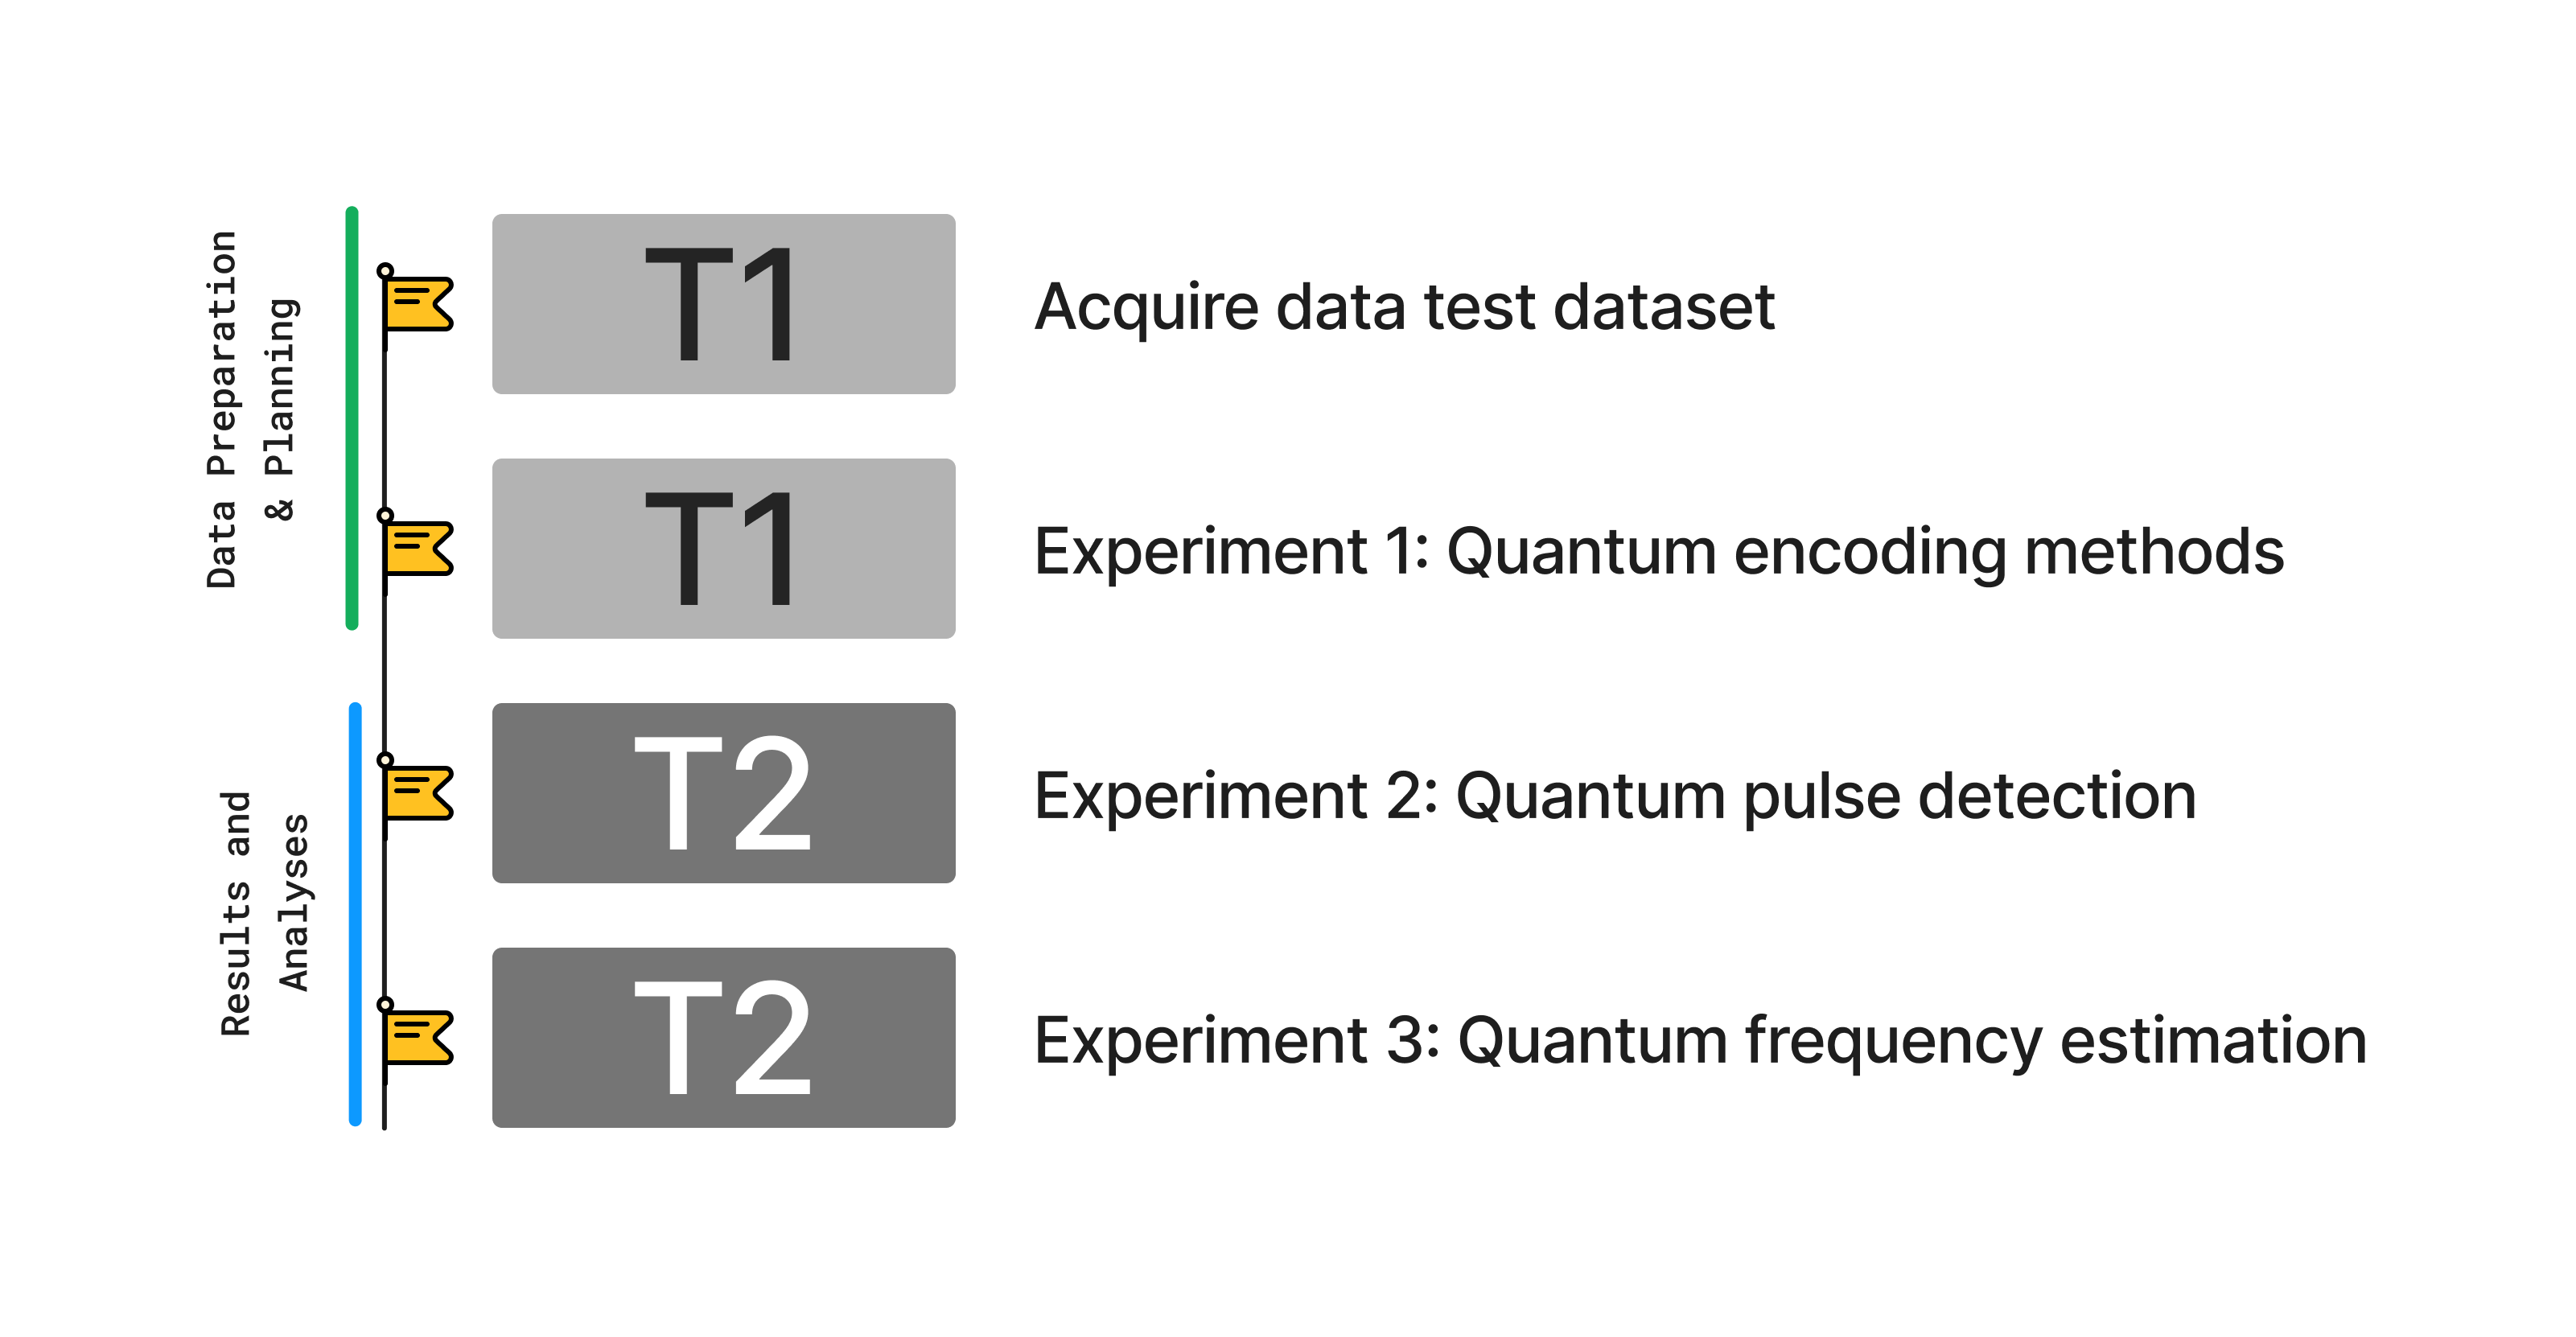
\includegraphics[width=1\textwidth]{Figures/roadmap.png}
    \caption{Research roadmap}
    \label{fig:roadmap}
\end{figure}
